%% ==========================================================================
%% OpenThomas -- ICAIF '26 submission version.
%% Double-blind review: acmart sigconf, anonymized, review line numbers.
%% Hard limit: <= 8 pages INCLUDING references (over-length = desk reject).
%%
%% CAMERA-READY TODO (revert for the final version):
%%   - remove the `anonymous` and `review` class options;
%%   - restore \settopmatter{printacmref=true} and the copyright permission
%%     block (delete the two suppression lines below);
%%   - fill \acmISBN / \acmDOI / \setcopyright, real author + affiliation;
%%   - restore the repository / project URLs (footnote below).
%% ==========================================================================
\documentclass[sigconf,review,anonymous]{acmart}

% -- Review-only space savers (RESTORE for camera-ready) --------------------
\settopmatter{printacmref=false}
\renewcommand\footnotetextcopyrightpermission[1]{}
\pagestyle{plain}

% -- Conference metadata (placeholders are fine for review) -----------------
\acmConference[ICAIF '26]{ACM International Conference on AI in Finance}{November 14--17, 2026}{Milan, Italy}
\acmYear{2026}
\copyrightyear{2026}

\usepackage{tikz}
\usetikzlibrary{arrows.meta, positioning, calc, fit, backgrounds}
\definecolor{detfill}{RGB}{224,236,247}
\definecolor{detline}{RGB}{70,120,170}
\definecolor{mdlfill}{RGB}{250,224,190}
\definecolor{mdlline}{RGB}{210,120,30}
\definecolor{srcfill}{RGB}{234,234,234}
\definecolor{srcline}{RGB}{120,120,120}

\begin{document}

\title{The Harness Is the Edge: A Disciplined, Self-Improving Language-Model
Agent for Weather Prediction Markets}

\author{Anonymous Author(s)}
\affiliation{%
  \institution{}
  \country{}
}

\begin{abstract}
Every frontier language model given real capital to trade prediction markets
autonomously has lost money. We argue this is a \emph{harness} problem, not a
forecasting-accuracy one: the profitable signature is selectivity, sized
asymmetry, exit discipline, and calibration --- properties of the system around
the model, not the model itself. We present \textbf{OpenThomas}, an open-source
agent built to be that harness and pointed at the one category where a harness is
measurable: daily station-temperature markets on Kalshi and Polymarket, which
settle daily against an objective public record (the U.S. National Weather
Service report for a named station). That makes them a \emph{strong-evaluator}
domain --- dense, objective, and reproducible in leak-free replay. OpenThomas
prices each strike from a seven-model numerical-weather-prediction consensus plus
its own GraphCast and GenCast forecasts, learns each station's systematic bias
from leak-free hindcasts, lets a language model make a \emph{bounded} adjustment,
blends with the market prior, and sizes with fractional Kelly under hard risk
limits the model cannot override. It also improves itself: an evolution loop
proposes bounded mutations that must clear a kernel-owned gate on leak-free
replay, with the evaluator kept off the agent's edit surface so self-improvement
cannot redefine ``improvement.'' In a 21-day replay on real order books with fees
(968 settled markets), a naked model-vs-market rule barely loses
(\$0.007/contract, 425 trades) while a market-prior blend turns expectancy
positive ($+$\$0.028) by trading less than half as often (184 trades):
selectivity, not the model, is the edge. We report the losing rows too.
Contributions: (i) the harness-is-the-edge thesis as a concrete, reproducible
system; (ii) a leak-free hindcast/replay methodology for market agents; and (iii)
a self-improvement architecture whose safety derives from keeping the judge off
the edit surface, evaluated on a domain with a strong judge.
\end{abstract}

\keywords{prediction markets, large language model agents, autonomous trading,
forecast calibration, numerical weather prediction, recursive self-improvement,
risk management}

\maketitle

\section{Introduction}

The obvious way to build a trading agent on top of a large language model (LLM)
is to ask the model what will happen and bet accordingly. The empirical record
says this does not work. The \emph{Prediction Arena} benchmark \cite{predarena}
gave six frontier models \$10{,}000 each and let them trade real prediction
markets autonomously for 57 days. Every one of them lost money, between $-16\%$
and $-30.8\%$. Research \emph{volume} had no correlation with returns; token
spend had none either. What separated the least-bad runs from the worst was not
a better world model but better \emph{behavior}: being right early, sizing up
when confident and down when uncertain, holding winners to settlement rather
than exiting early, and --- above all --- not trading at all when there was no
edge. The single profitable run on record ($+10.9\%$) was selective (112
trades), asymmetric (average win \$63.89 vs.\ average loss \$3.23), and
low-drawdown (4.1\%).

That profile is a property of the \emph{harness} --- the scaffolding that decides
when the model is allowed to act, how much, and under what constraints --- not of
the model's raw forecasting ability. Our central claim follows:

\begin{quote}
\emph{The LLM is not the edge. The harness is the edge.}
\end{quote}

This reframing has a sharp methodological consequence. If the edge lives in the
harness, then to make progress we need a domain where harness quality is
\emph{measurable} --- densely, objectively, and without leakage. Most prediction
markets fail this test: they settle rarely (one data point every few months),
their resolution is ambiguous, and any backtest risks letting the replayed market
``know'' something the replayed model did not. \textbf{Weather markets are the
exception.} A daily station-temperature market (``Will the high in Central Park
exceed 83\textdegree{}F today?'') resolves against the NWS climatological report
for one named station, every day, with no ambiguity. Dozens of ground-truth data
points arrive per day. This is the fastest, cleanest learning loop in prediction
markets, and it is what makes both the trading edge and, later, recursive
self-improvement, something you can put a number on.

We present \textbf{OpenThomas},\footnote{Open-source; the repository and live
project URLs are withheld here to preserve double-blind anonymity and will be
restored in the camera-ready version.} an open-source ($\approx$7{,}300 lines of
Python, 182 tests) autonomous agent that operationalizes the harness thesis on
weather markets. Its design commitments are:

\begin{itemize}
\item \textbf{Selectivity over activity.} ``No trade'' is the default action. The
agent trades only when $|\,\hat{p}-\text{price}\,|$ clears an explicit
expected-value threshold after fees and spread.
\item \textbf{A statistical baseline the model may adjust but never replace.}
Every strike is priced from a seven-model NWP consensus, corrected by
per-(station, lead) bias and spread learned from leak-free hindcasts, and hard-
truncated by what today's thermometer has already locked in. The LLM is clamped
to $\pm 0.15$ around this baseline.
\item \textbf{Hard risk constraints outside the model.} Fractional Kelly sizing,
per-market / per-event / per-category caps, a fee-aware EV threshold, a
longshot-zone filter, and a drawdown kill-switch are deterministic code. The
model proposes; the risk engine disposes.
\item \textbf{Calibration as a first-class metric,} tracked per (station, lead)
as Brier skill against the market, and used to license sizing only where skill is
positive.
\item \textbf{Self-improvement as a gated loop} in which the evaluator is
structurally off the agent's edit surface (Section~\ref{sec:rsi}).
\end{itemize}

We contribute: (1) the harness-is-the-edge thesis operationalized as a concrete
system, with an honest empirical account including the losing runs; (2) a
leak-free hindcast/replay methodology for evaluating market agents where the
replayed market is never allowed to know what the replayed model does not; and
(3) a self-improvement architecture whose safety comes from a kernel/agent plane
split that keeps the judge off the edit surface, stress-tested on a domain with a
genuinely strong judge.

\section{Background and related work}

\paragraph{LLMs as forecasters and traders.} A growing literature evaluates LLMs
as probabilistic forecasters. The consistent finding is that \emph{pure} LLM
forecasts underperform market consensus, but a \emph{blend} of the model with the
market price can beat the market \cite{blend}. Prediction Arena \cite{predarena}
extends this from forecasting to \emph{live autonomous trading} and finds uniform
losses, isolating behavioral rather than epistemic failure modes. Our work takes
the blend result and the behavioral diagnosis as design inputs: we blend with the
market prior by construction, and we push the behavioral factors (selectivity,
asymmetry, exit discipline) into deterministic code rather than prompting for
them.

\paragraph{Neural weather prediction.} Machine-learned global weather models now
match or exceed operational physics-based systems: GraphCast \cite{graphcast}
produces deterministic 10-day forecasts, and GenCast \cite{gencast} produces
calibrated ensembles via a diffusion sampler. These open-weights models run on
commodity accelerators. OpenThomas uses them as \emph{additional voters} in a
forecast consensus and, crucially, post-processes them per settlement station ---
the place where public global forecasts are systematically biased and where a
small, learnable, local correction becomes a durable edge.

\paragraph{Prediction-market microstructure.} The favorite--longshot bias ---
low-priced contracts are systematically overbet --- is well documented
\cite{longshot}; we encode it as a hard longshot-zone filter. Cross-venue listing
of the same real-world event (Polymarket vs.\ Kalshi) creates episodic
arbitrage, which our scanner flags deterministically.

\paragraph{Self-improving agents.} Recent framing of near-term recursive
self-improvement (RSI) locates the leverage not in model weights but in the
\emph{harness} --- how the agent plans, acts, remembers, and is evaluated --- and
identifies \emph{evaluator strength} as the first bottleneck \cite{harness}.
Open-ended methods such as the Darwin G\"odel Machine \cite{dgm} keep an archive
of past variants as mutation parents to resist diversity collapse. OpenThomas
adopts both ideas and adds a security model: because weather markets supply an
unusually strong evaluator, the risk is no longer a weak judge but a
\emph{gameable} one, so we make the judge structurally unwritable by the
optimizer.

\section{Why weather markets are a strong-evaluator domain}
\label{sec:weather}

Three properties make daily station-temperature markets uniquely suited to
measuring harness quality.

\textbf{Dense, objective settlement.} Each market resolves against the NWS
Climatological Report (product type \texttt{CLI}) for one named station, once per
day. There is a single number --- the day's observed maximum or minimum --- and no
interpretive latitude. A generalist prediction-market agent might see a few dozen
settlements per \emph{year}; a weather desk on ten U.S.\ cities (highs and lows)
sees dozens per \emph{day}.

\textbf{A learnable, local edge.} Markets settle on a \emph{specific} station
(NYC $=$ Central Park; Chicago $=$ Midway), and global forecast models have
systematic, station-specific biases there. Our first 90-day hindcast found the
Miami consensus running $1.8$--$2.1$\textdegree{}F cold ($\sigma\,1.7$),
Philadelphia $+2.3$\textdegree{}F, and LAX about $1$\textdegree{}F warm. These are
biases you can estimate from free public data, per station, offline --- a moat
that does not depend on privileged information, only on the discipline to measure
and apply it.

\textbf{Leak-free reproducibility.} Historical ``as-of'' forecast data (what a
model predicted at a past issue time) and historical order books are both
available, so a backtest can present the replayed agent with exactly the
information it would have had --- and no more. This is what lets us evaluate not
just the forecast but the \emph{decision rule}, and later, self-improvement,
without the replay silently cheating. The same three properties are what the RSI
literature asks for and rarely gets: an objective, dense, reproducible evaluator
\cite{harness}.

\section{System architecture}
\label{sec:arch}

OpenThomas is organized as a stack of layers with a strict rule about who is in
control at each one (Figure~\ref{fig:pipeline}, Table~\ref{tab:layers}).
Everything that touches money --- sizing and exposure --- is deterministic code;
the language model is confined to a bounded adjustment in the middle of the
pipeline.

\begin{figure*}[t]
\centering
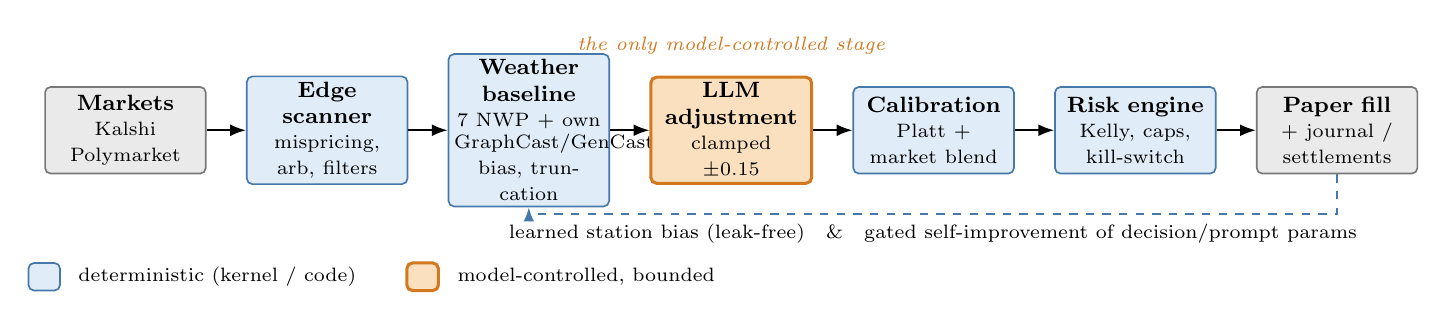
\begin{tikzpicture}[
  font=\footnotesize,
  box/.style={draw, rounded corners=2pt, align=center, minimum height=11mm,
              inner sep=2pt, text width=19mm, line width=0.6pt},
  det/.style={box, fill=detfill, draw=detline},
  mdl/.style={box, fill=mdlfill, draw=mdlline, line width=1.1pt},
  src/.style={box, fill=srcfill, draw=srcline},
  flow/.style={-{Latex[length=2mm]}, line width=0.7pt},
  fb/.style={-{Latex[length=1.8mm]}, dashed, line width=0.7pt, draw=detline},
  node distance=5mm,
]
\node[src] (mk) {\textbf{Markets}\\[1pt]\scriptsize Kalshi\\\scriptsize Polymarket};
\node[det, right=of mk] (scan) {\textbf{Edge}\\\textbf{scanner}\\[1pt]\scriptsize mispricing,\\\scriptsize arb, filters};
\node[det, right=of scan] (base) {\textbf{Weather}\\\textbf{baseline}\\[1pt]\scriptsize 7 NWP + own\\\scriptsize GraphCast/GenCast,\\\scriptsize bias, truncation};
\node[mdl, right=of base] (llm) {\textbf{LLM}\\\textbf{adjustment}\\[1pt]\scriptsize clamped\\\scriptsize $\pm 0.15$};
\node[det, right=of llm] (cal) {\textbf{Calibration}\\[1pt]\scriptsize Platt +\\\scriptsize market blend};
\node[det, right=of cal] (risk) {\textbf{Risk engine}\\[1pt]\scriptsize Kelly, caps,\\\scriptsize kill-switch};
\node[src, right=of risk] (fill) {\textbf{Paper fill}\\[1pt]\scriptsize + journal /\\\scriptsize settlements};

\foreach \a/\b in {mk/scan, scan/base, base/llm, llm/cal, cal/risk, risk/fill}
  \draw[flow] (\a) -- (\b);

% learning feedback: settlements teach the baseline (leak-free), gate the params
\draw[fb] (fill.south) -- ++(0,-5mm) -| node[pos=0.25, below, font=\scriptsize]
  {learned station bias (leak-free) \; \& \; gated self-improvement of decision/prompt params} (base.south);

% highlight: the single model-controlled stage
\node[mdlline, font=\scriptsize\itshape, above=1.5mm of llm] {the only model-controlled stage};

% legend
\begin{scope}[shift={($(mk.south west)+(0,-13mm)$)}]
  \node[det, minimum height=3.5mm, minimum width=4mm, text width=0pt, inner sep=0pt] (l1) {};
  \node[right=1mm of l1, font=\scriptsize] (l1t) {deterministic (kernel / code)};
  \node[mdl, right=5mm of l1t, minimum height=3.5mm, minimum width=4mm, text width=0pt, inner sep=0pt] (l2) {};
  \node[right=1mm of l2, font=\scriptsize] {model-controlled, bounded};
\end{scope}
\end{tikzpicture}
\caption{The OpenThomas pipeline. A trade flows left to right; only one stage
is model-controlled, and it is clamped to the statistical baseline $\pm 0.15$
and bracketed by deterministic layers on both sides. Settled outcomes feed back
to teach the baseline each station's bias (strictly leak-free) and to gate
self-improvement of the decision and forecast-prompt parameters. Sizing and
exposure never leave deterministic code.}
\label{fig:pipeline}
\end{figure*}

\begin{table*}[t]
\centering
\small
\begin{tabular}{@{}p{2.4cm}p{10.2cm}p{2.9cm}@{}}
\toprule
\textbf{Layer} & \textbf{What it does} & \textbf{Who's in control} \\
\midrule
Edge scanner & Filters markets to plausible mispricings; flags cross-venue arbitrage and longshot / resolution-trap zones & deterministic code \\
Weather baseline & Seven-model NWP consensus $+$ own GraphCast/GenCast $\to$ per-strike probability at the settlement station, with per-(station, lead) bias/$\sigma$ from leak-free hindcasts and hard truncation by today's observed extreme & deterministic code \\
Forecast engine & LLM ensemble (median of $N$ independent estimates), grounded in resolution rules and base rates, \emph{clamped to baseline $\pm 0.15$} & your choice of model \\
Calibration & Platt-scales forecasts against your own settled history; blends with the market prior & deterministic code \\
Risk engine & Fractional Kelly, per-market/event/category caps, fee-aware EV threshold, longshot filter, drawdown kill-switch & deterministic code \\
Memory & Every forecast and fill journaled to SQLite; post-settlement reflection distills bounded playbook rules & agent, human-auditable \\
\bottomrule
\end{tabular}
\caption{The OpenThomas stack. The model \emph{proposes}; the risk engine
\emph{disposes}. Only one layer is model-controlled, and it is bounded above and
below by deterministic layers.}
\label{tab:layers}
\end{table*}

\paragraph{Market connectors and paper simulation.}
A unified \texttt{Market}/\texttt{Order}/\texttt{Position} model spans Polymarket
(Gamma API for discovery, CLOB for books/orders) and Kalshi (REST $+$ WebSocket,
RSA-signed, CFTC-regulated). A \emph{paper} connector wraps either venue's real
market data but simulates fills locally at bid/ask (never mid), with
mark-to-market at bid prices (liquidation value, not hope). Paper mode is the
default and needs no exchange keys, which makes the whole system runnable --- and
reproducible --- by anyone.

\paragraph{The weather baseline.}
For a market on station $s$, valid day $d$, kind $k\in\{\text{high},\text{low}\}$,
the baseline forms a consensus temperature $\bar{T}$ across seven operational
global models (GFS, ECMWF-IFS, ICON, GEM, UKMO, M\'et\'eo-France, JMA) plus the
system's own GraphCast point forecast, with a cross-model spread
$\sigma_{\text{model}}$. It then applies two corrections learned strictly
out-of-window:
\[
\hat{T} = \bar{T} + b_{s,k,\ell}, \qquad
\sigma^2 = \sigma_{\text{model}}^2 + \sigma_{s,k,\ell}^2 ,
\]
where $\ell$ is the forecast lead, $b_{s,k,\ell}$ the learned station bias and
$\sigma_{s,k,\ell}$ its residual spread. GenCast contributes a
\emph{flow-dependent} multiplier on $\sigma$ (an uncertain synoptic setup widens
the distribution) rather than a point estimate, because its 12-hour steps
undersample the diurnal peak. The per-strike probability is then the Gaussian (or
empirical) mass on the correct side of the strike, with one more hard step:
\emph{truncation}. If today's thermometer has already recorded a value that makes
one side of the strike impossible (the observed high already exceeds the floor),
the probability is clamped accordingly. This is where a naive backtest leaks, and
where Section~\ref{sec:eval} spends most of its care.

\paragraph{Forecast engine: bounded LLM adjustment.}
The language model's role is deliberately small. It receives the baseline
probability, the resolution rules, base rates, and a news brief, and returns an
adjusted probability --- which is then \emph{clamped to baseline $\pm 0.15$}. The
statistics do the heavy lifting; the model is there for what the statistics cannot
see (a blown front, a stale consensus, a discontinuity in the question text), not
to substitute its own guess for a calibrated ensemble. Because of the clamp,
mid-size local reasoning models suffice, which keeps the agent runnable on
self-hosted open-weights models with no API bill and full privacy. The engine
takes the median of $N$ independent estimates under different framings to reduce
single-sample variance.

\paragraph{Calibration and market-prior blend.}
Once $\geq 30$ markets settle in a category, OpenThomas fits Platt scaling to
correct the model's systematic over/under-confidence, then blends the calibrated
forecast with the market price. The blend is not a hedge --- it is the empirically
supported position that a model--market blend beats either alone \cite{blend}. The
blend weight is an entry-\emph{selectivity} parameter (how much to trust our view
vs.\ the crowd), and as such is a candidate for self-improvement under kernel
bounds (Section~\ref{sec:rsi}); the sizing that follows is not.

\paragraph{Risk engine (deterministic).}
The risk engine takes bankroll, risk profile, the (blended) probability and
confidence, and market price/liquidity, and returns an approved size or a
rejection naming the binding constraint. It applies fractional Kelly (profile-
scaled $0.15\times$--$0.33\times$), per-market concentration caps, per-category
and per-event correlation caps (correlated settlements produced Prediction
Arena's largest single-session losses), a fee-aware EV threshold, a longshot-zone
filter, a solvency check including fees, and a drawdown kill-switch that halts
trading and requires a human to resume. None of these are reachable by the model
or by the self-improvement loop; a kernel policy test fails any change that tries
to move a safety rail into the optimizer's reach.

\section{Self-improvement with the judge off the edit surface}
\label{sec:rsi}

OpenThomas updates OpenThomas. The operator (a human, or a coding assistant) is
moved \emph{up} the stack --- setting bounds and reviewing lineage --- and is
forbidden from hand-tuning trading parameters; that is what the evolution loop is
for. The design problem is that self-improvement is safe only if improvement
cannot redefine ``improvement.'' An optimizer that can edit its own judge will
find it easier to lower the bar than to clear it.

\paragraph{Kernel/agent planes.} The codebase is split into two planes, and the
split \emph{is} the security model (Table~\ref{tab:planes}). The \textbf{kernel}
plane --- promotion gate, parameter bounds, the risk engine and all safety rails,
the truth pipeline, the journal schema --- is written only by the operator; the
evolution loop has no write path to it. The \textbf{agent} plane --- decision-rule
parameters, the forecast prompt template, and (on the roadmap) workflow structure,
strategy code, and the evolver itself --- is written by the evolution loop, but
only \emph{through} the kernel gate. The line is drawn precisely:
entry-selectivity knobs (minimum edge, market-prior blend weight) are genome
parameters under kernel bounds, while sizing, exposure caps, and the kill-switch
can never enter the parameter space.

\begin{table}[t]
\centering
\small
\begin{tabular}{@{}p{1.3cm}p{4.2cm}p{1.7cm}@{}}
\toprule
\textbf{Plane} & \textbf{Contents} & \textbf{Written by} \\
\midrule
kernel & bounds, promotion gate, risk engine \& safety rails, truth pipeline, journal schema & operator only \\
agent & decision-rule params, forecast prompt template; later: workflow, strategy code, the evolver & evolution loop, \emph{via the gate} \\
\bottomrule
\end{tabular}
\caption{The plane split is the security model: the judge is not on the
optimizer's edit surface.}
\label{tab:planes}
\end{table}

\paragraph{Three nested loops.} A fast \emph{trading} loop (minutes) runs the
champion parameters and never waits on anything below it. A \emph{reflection} loop
(on settlements) distills bounded playbook rules. An \emph{evolution} loop mines
failure evidence from the journal, proposes mutations --- LLM-directed by the
evidence, plus Gaussian mutations drawn from an \emph{archive} of past variants
(Darwin G\"odel Machine-style, against diversity collapse \cite{dgm}) --- and
submits them to the gate.

\paragraph{The gate (kernel, frozen).} A candidate is a \emph{strategy callable}
scored on leak-free replay with four anti-gaming properties:
\emph{held-in/held-out} splits (winners are picked on older days; the freshest
settled days only get a veto, and the window rolls forward daily so repeated
meta-cycles face new data); \emph{totals-not-ratios} scoring with a minimum trade
count (a rule that trades twice cannot win on ratio; a rule that trades nothing
cannot win on drawdown); \emph{out-of-sample regret rollback} (each cycle first
re-scores the active generation against its parent on the fresh window and reverts
if the parent now wins); and a \emph{Brier veto} for the forecast operator (a
prompt that wins PnL while worsening calibration got lucky, and luck does not
promote). Generation 0 is the operator's config and applies no overrides --- the
human's settings win until the loop has promoted evidence-backed changes past
them.

\paragraph{One gate, growing write surface.} Improvement axes are unified as
mutation operators feeding the \emph{same} accept mechanism: playbook rules and
calibration refits (shipped), decision-parameter mutation and forecast-prompt
mutation (shipped), then workflow structure, then agent-plane code diffs (which
add shadow paper-trading and human diff review), then LoRA/GRPO weight updates
with a time-discounted reward $R\cdot e^{-\lambda\,\text{days-to-close}}$ --- a
trained adapter is just another candidate at the same gate. The admission rule is
strict: a parameter enters the space only when the gate can actually discriminate
on it. \emph{Tuning what you cannot measure is drift, not improvement.} This is
why code diffs come last --- they need the strongest evaluation (replay \emph{plus}
shadow trading \emph{plus} human review of the diff) --- and why the whole
enterprise is anchored to a domain with a strong evaluator in the first place.

\section{Leak-free evaluation methodology}
\label{sec:eval}

The hardest part of evaluating a market agent is not computing PnL; it is not
lying to yourself. Two commands encode the discipline. \texttt{hindcast} teaches
the baseline each station's bias from historical as-of forecasts and official
settlements, strictly \emph{before} any trading window it will be evaluated on.
\texttt{replay} then backtests the \emph{decision rule} against real historical
order books, drawing prices from snapshot candlesticks that \emph{precede} the
temperature extreme being bet on, with station bias/$\sigma$ learned only
out-of-window. The governing rule, learned the hard way when an early backtest
snapshotted the dawn low after it had already been realized: \emph{never let the
replayed market know something the replayed model does not.} A single timing leak
turned a losing strategy into a fake winner; fixing it turned it back. This
methodology is what makes the self-improvement gate trustworthy: the same
row-collection pipeline that scores a candidate generation is the one that
enforces no-peeking, and it lives in the kernel where the optimizer cannot touch
it.

\section{Empirical results}
\label{sec:results}

We report an ablation from a 21-day leak-free replay on real Kalshi order books
with fees included (Table~\ref{tab:ablation}); the window covers 968 settled
markets with settlement dates from 2026-06-24 to 07-14. These are small-sample,
paper-mode numbers on a baseline \emph{deliberately stripped} of every live-only
advantage (same-day model runs, intraday observations, LLM adjustment, and the
calibration layer); they are an existence proof about \emph{where the edge comes
from}, not a track record. The live agent trades with all four advantages on, and
whether they clear the bar is precisely what the public paper run exists to
answer.

\begin{table}[t]
\centering
\small
\begin{tabular}{@{}p{4.15cm}rrr@{}}
\toprule
\textbf{Decision rule (21-day replay)} & \textbf{Trades} & \textbf{Win} & \textbf{PnL/ct} \\
\midrule
Naked model-vs-market & 425 & 41\% & $-\$0.007$ \\
\quad $+$ learned station bias & 396 & 39\% & $-\$0.005$ \\
\quad\quad $+$ market-prior blend (production) & 184 & 45\% & $+\$0.028$ \\
\bottomrule
\end{tabular}
\caption{Leak-free replay over 968 settled markets (2026-06-24 to 07-14; fees in;
timing-safe snapshots --- lows 06Z, highs 15Z; station bias learned strictly
out-of-window). The market-prior blend more than halves activity
($425\!\to\!184$ trades) and flips expectancy positive: \emph{selectivity}, not
the model, is the edge. The naked rule barely clears zero because the late-morning
book has already priced the day's early observations.}
\label{tab:ablation}
\end{table}

Two findings are worth drawing out. First, the naked model-vs-market rule
\emph{loses} ($-\$0.007$/contract over 425 trades): by late morning the order book
has already digested the day's early observations, so the raw model has almost
nothing to add --- exactly the ``the model is not the edge'' prediction, borne out
on real books. Second, the edge is recovered not by a sharper forecast but by
\emph{selectivity}: blending the model with the market prior more than halves
activity ($425\!\to\!184$ trades) and flips expectancy to $+\$0.028$/contract at a
45\% win rate, i.e.\ the surviving trades pay asymmetrically. Learned station bias
adds a smaller, consistent nudge ($-\$0.007\!\to\!-\$0.005$); the 90-day hindcast
that supplies it recovers stable, station-specific biases (Miami
$+1.8$--$2.1$\textdegree{}F, Philadelphia $+2.3$, LAX $-1$) that persist
out-of-sample.

We report the losing rows next to the positive one, and stress the caveats: 184
trades over three weeks in paper mode is an existence proof, not a track record,
and a single window can flatter a rule. The honest claim is narrow and, we think,
more useful than a headline return: on weather markets the structural edges are
\emph{real but small}, discipline --- selectivity and blending with the crowd, not
a smarter model --- is what realizes them, and this is the market category where
that statement can be checked.

\section{Discussion and limitations}

\paragraph{Small samples, paper mode.} The replay is 21 days and simulated at real
bid/ask; it is an ablation, not a track record. The reference agent's live paper
run is the ongoing, public test, reported with wins and losses alike.

\paragraph{Capacity is the real ceiling.} Daily-temperature markets are thin. A
survey of seven Kalshi cities found on the order of a few hundred thousand dollars
of daily notional in aggregate, which bounds extraction at low-single-digit
millions per year even under optimistic assumptions. This is a research and
methodology contribution about \emph{measurable} edge, not a claim of scalable
returns.

\paragraph{Replay fidelity.} Replay has no news brief, no intraday observations,
no forecaster-discussion text, and no calibration layer; it measures the
template's skill at adjusting the statistical baseline, which is the dominant live
pathway for weather markets, but it is not the whole live agent. A residual leak
risk --- an LLM ``remembering'' recent weather from pre-training --- is negligible
with a local model whose cutoff precedes the window, but must be rechecked
whenever the forecaster is swapped.

\paragraph{Generalization.} The strong-evaluator property is what makes weather
the right first domain; it is also what most other markets lack. Extending the
harness (and the self-improvement gate) to weaker-evaluator markets is future
work, and the journal already archives each live forecast's inputs so that a
future trace-replay evaluator can begin to close that gap.

\section{Reproducibility, ethics, and broader impact}

The system, the evaluation harness, and the reference agent's live feed are
public; paper mode requires no exchange keys and reproduces the replay numbers
from public data. Live trading is off by default and requires two independent
explicit opt-ins; the agent has no deposit, withdrawal, or transfer capability and
can only trade within an allocated bankroll. We ship hard position limits and a
drawdown kill-switch, and we state plainly that no software makes trading safe:
roughly 70\% of Polymarket addresses have lost money, and every layer of this
paper is about losing less, not winning easily. On the self-improvement side, the
safety argument is architectural rather than behavioral: the judge is off the
optimizer's edit surface by construction, safety rails are outside the parameter
space by a kernel policy test, and every future promotion is an auditable commit
authored by the loop itself.

\section{Conclusion}

Autonomous LLM traders lose money not because they forecast badly but because they
lack discipline. OpenThomas puts the discipline in deterministic code, uses a
language model only for a bounded adjustment it is well-suited to, and points the
whole system at weather markets --- the one category where the resulting edge, and
the system's ongoing self-improvement, can be measured densely, objectively, and
without leakage. The edge we find is real, small, and preserved by discipline. We
report it in public, losses included, and we invite the community to check it.

\begin{thebibliography}{9}
\bibitem{predarena} Prediction Arena: evaluating frontier language models as
autonomous prediction-market traders. arXiv:2604.07355, 2026.
\bibitem{blend} Calibrated LLM forecasts and market-prior blending.
arXiv:2511.07678, 2025.
\bibitem{graphcast} R.~Lam et al. GraphCast: Learning skillful medium-range global
weather forecasting. \emph{Science}, 382(6677):1416--1421, 2023.
\bibitem{gencast} I.~Price et al. Probabilistic weather forecasting with machine
learning. \emph{Nature}, 637:84--90, 2025.
\bibitem{longshot} J.~Whelan et al. The favorite--longshot bias in prediction
markets. SSRN 5502658, 2026.
\bibitem{harness} L.~Weng. Harness Engineering for Self-Improvement. Blog post,
2026.
\bibitem{dgm} The Darwin G\"odel Machine: open-ended self-improvement with a
variant archive. 2025.
\end{thebibliography}

\end{document}
